%\documentclass{acm_proc_article-sp} 
\documentclass[14pt]{article} 
\usepackage{amssymb,amsmath} 
\usepackage{setspace}
\usepackage{graphicx}
\usepackage{float}
\usepackage{hyperref}

\doublespacing


\floatstyle{ruled}
\newfloat{code}{thp}{lop}
\floatname{code}{Code}

%\DeclareGraphicsExtensions{.eps}

\begin{document}
	
\title{DBToaster Runtime: A System for Streaming Data Processing. \\And\\ AlgoTrader: A Trading Algorithms Platform for Stock Exchange Simulation.}
\author{}
\maketitle

\section{Introduction}

DBToaster application involves three major components. Data Sources components are a source of the incoming data. The end user applications need these data to be processed by running various queries over it. In this particular example we will be using an Exchange Simulation Server application as a data source. Next component is the Algorithms Simulation Engine. This component is the end user program of interest. It is responsible for the decision making and outside influences (i.e. what ever user needs to be done with the help of the queries over the data streams). In out example it is a Trading Runtime Platform. The last component is DBToaster Runtime. The component is responsible for collecting the data from various data sources specified by the users, running appropriate queries over the data and conveying the query results to Algorithms Simulation Engine. 

The the flow of information between the three components is as follows. Once started data generation component generates data, these data comes from a variety of sources stock exchange, sensor network, remote applications etc. The data comes as a continuous stream of information, this information is presented in a well known format. In many of the cases it is possible that the end user does not have much control over the data stream but the ability to listen to the incoming data. These data is sent to DBToaster runtime. The runtime is responsible for collecting data from those data sources and running a dynamic set of user defined queries over these data. The queries are dynamically loaded, compiled and if needed removed during the execution of a runtime. The results of the queries are forwarded to Algorithms Simulation Engine (a.k.a the end user). The Engine's job is to get the data from the runtime. Based on the results of the queries Algorithm Engine performs tasks needed by the users. In our example, based on the information received Algorithm Engine buys and sell stocks on a NASDAQ exchange simulator. 

The particular application we have chosen to demonstrate the capabilities and performance of our system is a NASDAQ trading simulation. In this simulation there is a set of servers; each server arranges stock exchanges between different trading parties. The results of those exchanges as well as information about interest in stock sells and purchases is transmitted to all parties interested in such information. Based on these information different trading algorithms decide to buy and sell stocks. The arrangement of all the components in the Trading system can be seen in figure \ref{TheBigPicture}. 

\begin{figure}
  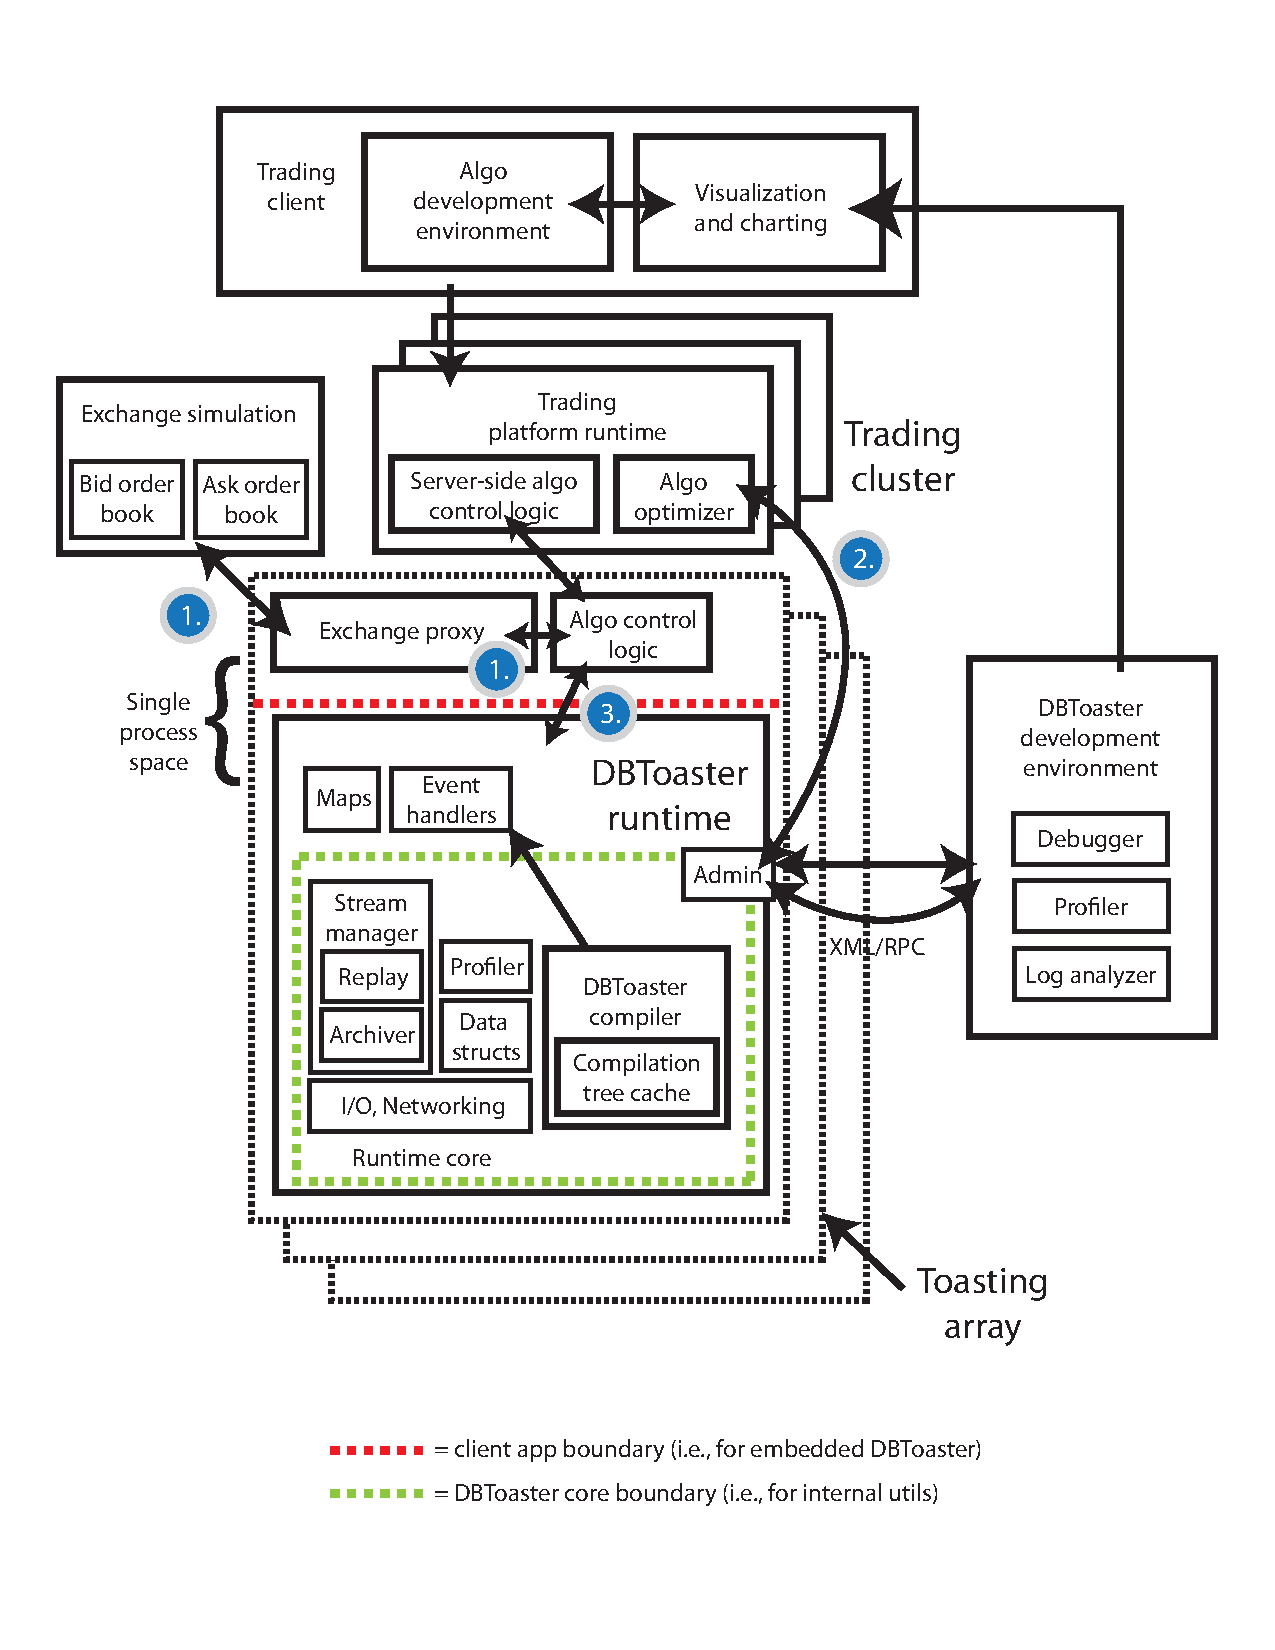
\includegraphics[width=4.50in]{../figures/finapp.pdf}
  \caption{Application Overview.}
  \label{TheBigPicture}
\end{figure}

%description of particularities of the system


\section{DBToaster Runtime}

DBToaster Runtime consists of three major components: Compiler, Query Processor and Data Sources Processor. Each of these components interacts with each other as well as has external interactions. The complete representation of DBToaster Runtime can be found in figure \ref{DBToasterPic}. Compiler and Query Processor have a server connection to handle user requests. Data Source Processor creates user specified clients to receive the data from various data sources. Compiler receives requests from the client to instantiate a Data Source Reader for receiving data or a SQL query to process data. The created Data Reader is passed to the Data Source Processor and a Query is passed to Query Processor to run on the data. 

\begin{figure}
  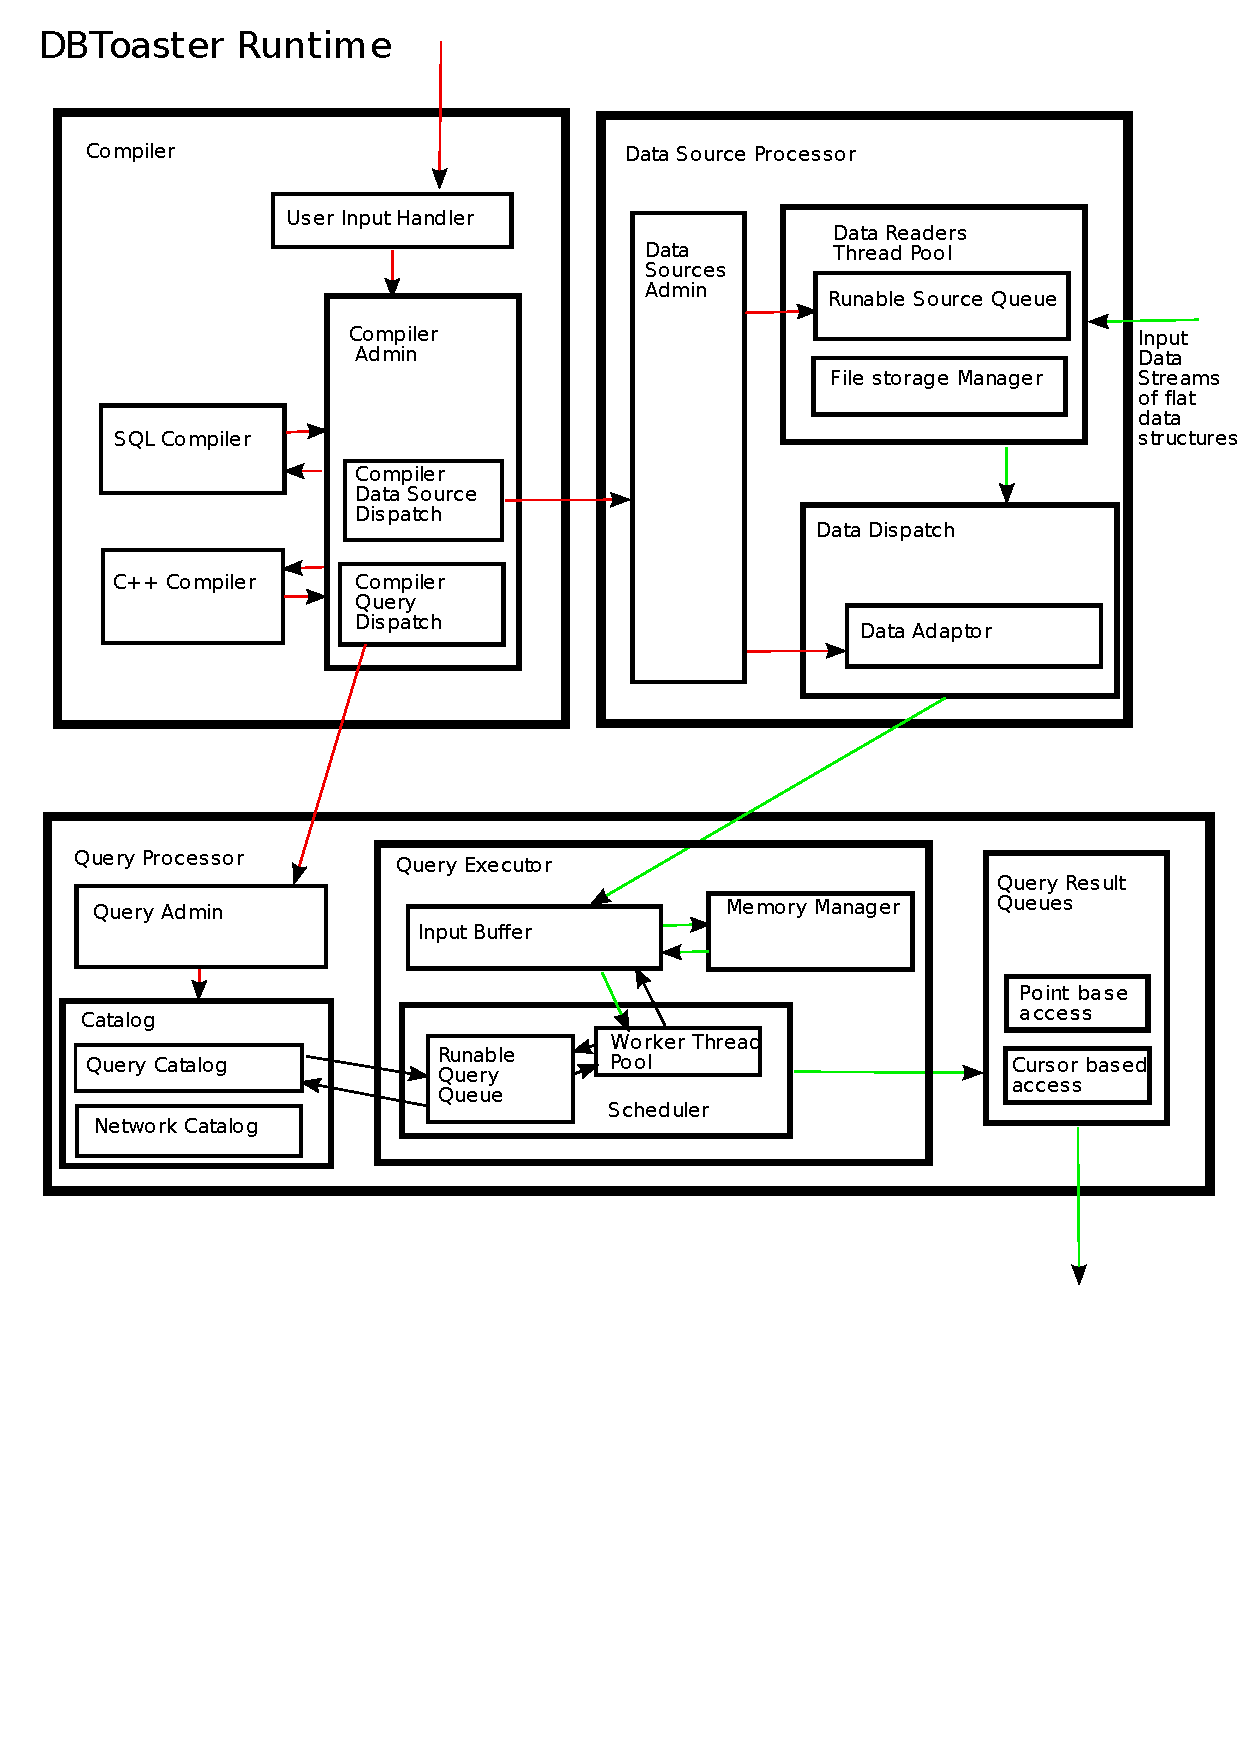
\includegraphics[width=4.50in]{../figures/DBToasterRuntime.pdf}
  \caption{DBToaster Structure.}
  \label{DBToasterPic}
\end{figure}



\subsection{Compiler}

Compiler consists of several components. Its structure can be seen in figure \ref{CompilerPicture}. Two components responsible for compilation are SQL query pre-compiler and C++ code compiler. 

Compiler is a starting point for all user interactions with the DBToaster Runtime. Once Runtime is up and running the user initiates the contact by specifying that they need to execute a query on some specific set of data sources. The query, types and parameters of data sources are sent to User Input Handler. The Input Handler collects the information in a structured format and passes it to the Compiler Admin. Compiler Admin converts a SQL query to C++ code and C++ code to binary format. The query is then passed to the Query Admin to be added to the list of active queries. If the user asks to add a Data Source Reader. The Reader of a specified type is created and passed to the Data Sources Admin to be added to the list of active Readers. The Data Adapter is compiled into a binary format and sent to Data Sources Admin to be added to Data Adaptors. 

\begin{figure}
  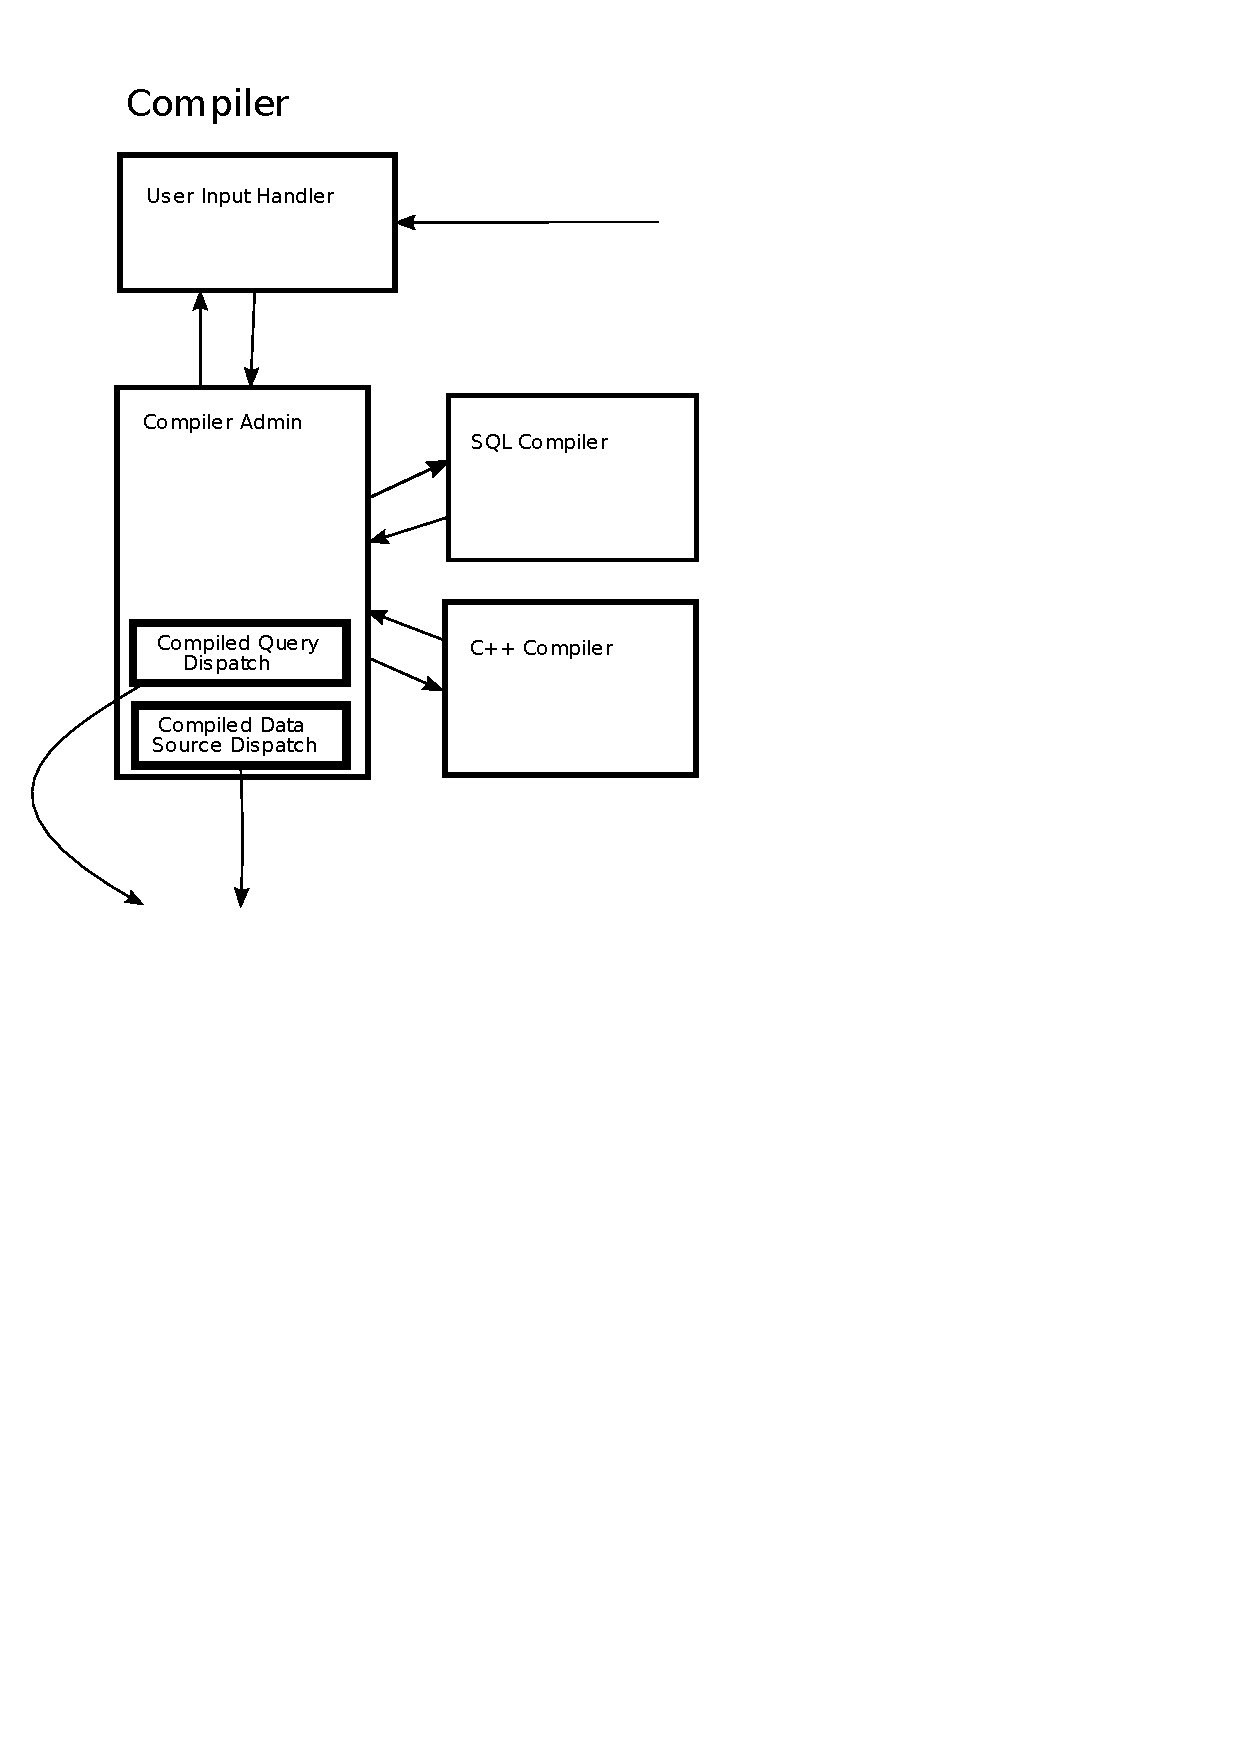
\includegraphics[width=4.50in]{../figures/compiler.pdf}
  \caption{Compiler Structure.}
  \label{CompilerPicture}
\end{figure}

\subsubsection{User Input Handler}
User Input Handler implements a server to respond to client requests. When a client connects to the Input Handler Server it sends a type of request and attributes of the request to the server:
\\
\\
\begin{tabular}{|l|l|}
  \hline
  Type & Request Attributes \\ \hline
  Query & Query Source file, list of Data Readers \\ \hline
  Reader & Connection Type, Adapter Source file \\ \hline
\end{tabular}
\\
\\*
The two different types of requests are either to add a query or add a data reader.
\\*
Add query request needs the following data from the user:

\begin{itemize}
	\item {\tt AddRequest(type="add query",\\
		 Source="SQL Source File",\\
	     DataReaders="list of Data Reader's IDs for Query");}
\end{itemize}

\noindent Add data reader request is as follows:

\begin{itemize}
	\item {\tt AddRequest(type="add reader", \\
	     AdaptorSource="C++ Adaptor Source file",\\
	     source="IPaddress and port or data input file");}
\end{itemize}

This information is then forwarded to the Compiler Admin in a form of a struct:

\begin{itemize}
	\item {\tt Struct InputRequest( int type, string fileName,\\
	       list<int> informationSources \\
		   list<string> sourceParameters)}
\end{itemize}

User Input Handler is implemented as a class with a server hidden inside. For now Input Handler also contains Compiler Admin. Compiler Admin can be abstracted to run in a separate thread. 

\subsubsection{Compiler Admin}

Once user request is received, Compiler Admin takes over. Depending on the type of the request Admin takes different actions. 

On add SQL query request Admin passes the SQL query source file to SQL Compiler. SQL compiler returns a pointer to an containing equivalent to a query C++ file. This file is then passed to the C++ compiler by the Admin. C++ compiler returns a function handle to the compiled binary of the query. The query handle is then passed to the Query Admin to be added to the catalog together with the list of Readers for the query.

On add Reader request Admin passes Data Adaptor file to C++ compiler which in turn returns a function handle to the Data Adaptor. Then Admin creates a Reader and opens a connection for a reader (either a socket or a file). The handle to a Reader together with the handle for a Data Adaptor and a list of queries for this reader is passed to the Data Sources Admin. 

\noindent Compiler Admin class looks as follows:
\begin{verbatim}
class CompilerAdmin
{
    void RunAdmin(InputRequest);

private:
    cCodeFileName  CompileSQL(string SQL_file_name);
    functionHandle CompileC++(string C++_file_name);
	
    SQLCompiler;
    CCompiler;
    QueryAdmin *;
    DataSourcesAdmin*;
}
\end{verbatim}

Method {\tt RunAdmin(InputRequest)} takes a user request to add a query or a data source. Compiler Admin contains a SQL Compiler and C++ compiler. It also contains pointers to Query Admin and Data Sources Admin to pass compiled handlers to them.

\subsubsection{SQL Compiler}

SQL complier takes a SQL query from a file and creates an optimized C++ coded to be added to the runtime. The file name containing the code is returned to the Admin.

\begin{itemize}
	\item {\tt cCodeFileName CompileSQL(SQL file name);}
\end{itemize}

\subsubsection{C++ Compiler}

C++ compiler takes file containing C++ code. C++ compiler creates a binary code version of the code and returns a function handle of it to Admin. \emph{not sure about the return form. it is possible we need to return several function handles ... not sure yet}

\begin{itemize}
	\item {\tt functionHandle CompileC++(C++ file name);}
\end{itemize}

\subsection{Data Source Processor}

\noindent Data Source Processing is done in two steps. Data Sources Admin receives two function handles from Compiler Admin a source reader and a data adaptor. 

\begin{itemize}
\item Source Reader handle is inserted into Collection of Data Sources. It processes outside data streams and forwards received information to data dispatcher.
\item Data Adaptor handle is inserted into a data dispatcher. Data Adaptor transforms received data into a format needed by the query.
\end{itemize} 

Data Sources Thread Pool stores threads and a collection of Source Readers. Each thread 

\begin{itemize}
	\item Picks a Source Reader from a collection
	\item Performs a data read 
	\item Forwards read data tuple to Data Dispatcher
\end{itemize}

\noindent The details of Data Source Processor can be seen in figure \ref{DataSourcePic}.

%where each thread picks a Data Reader and executes a read at a time from one of them. Once read is done the results of the read are forwarded to a Data Structure Dispatch. The Dispatch uses the appropriate Data Adapter to handle the data into a structured format, then the structured data is forwarded to Query Processor, in particular to the Query Tuple Queue. The more pictorial description can be found in figure \ref{DataSourcePic}.

% processing consists of the list of list of stream points. Each point is given by the user and signifies a way for a DBToaster to connect with the input stream of some process which dispatches data to the DBToaster. Each Stream Point is written by the user and user can fully specify how the data should be received and processed. Stream point is responsible for sending data to the Data Dispatch unite in a pre-specified format. The structure for data source processing can be found in figure 

\begin{figure}
  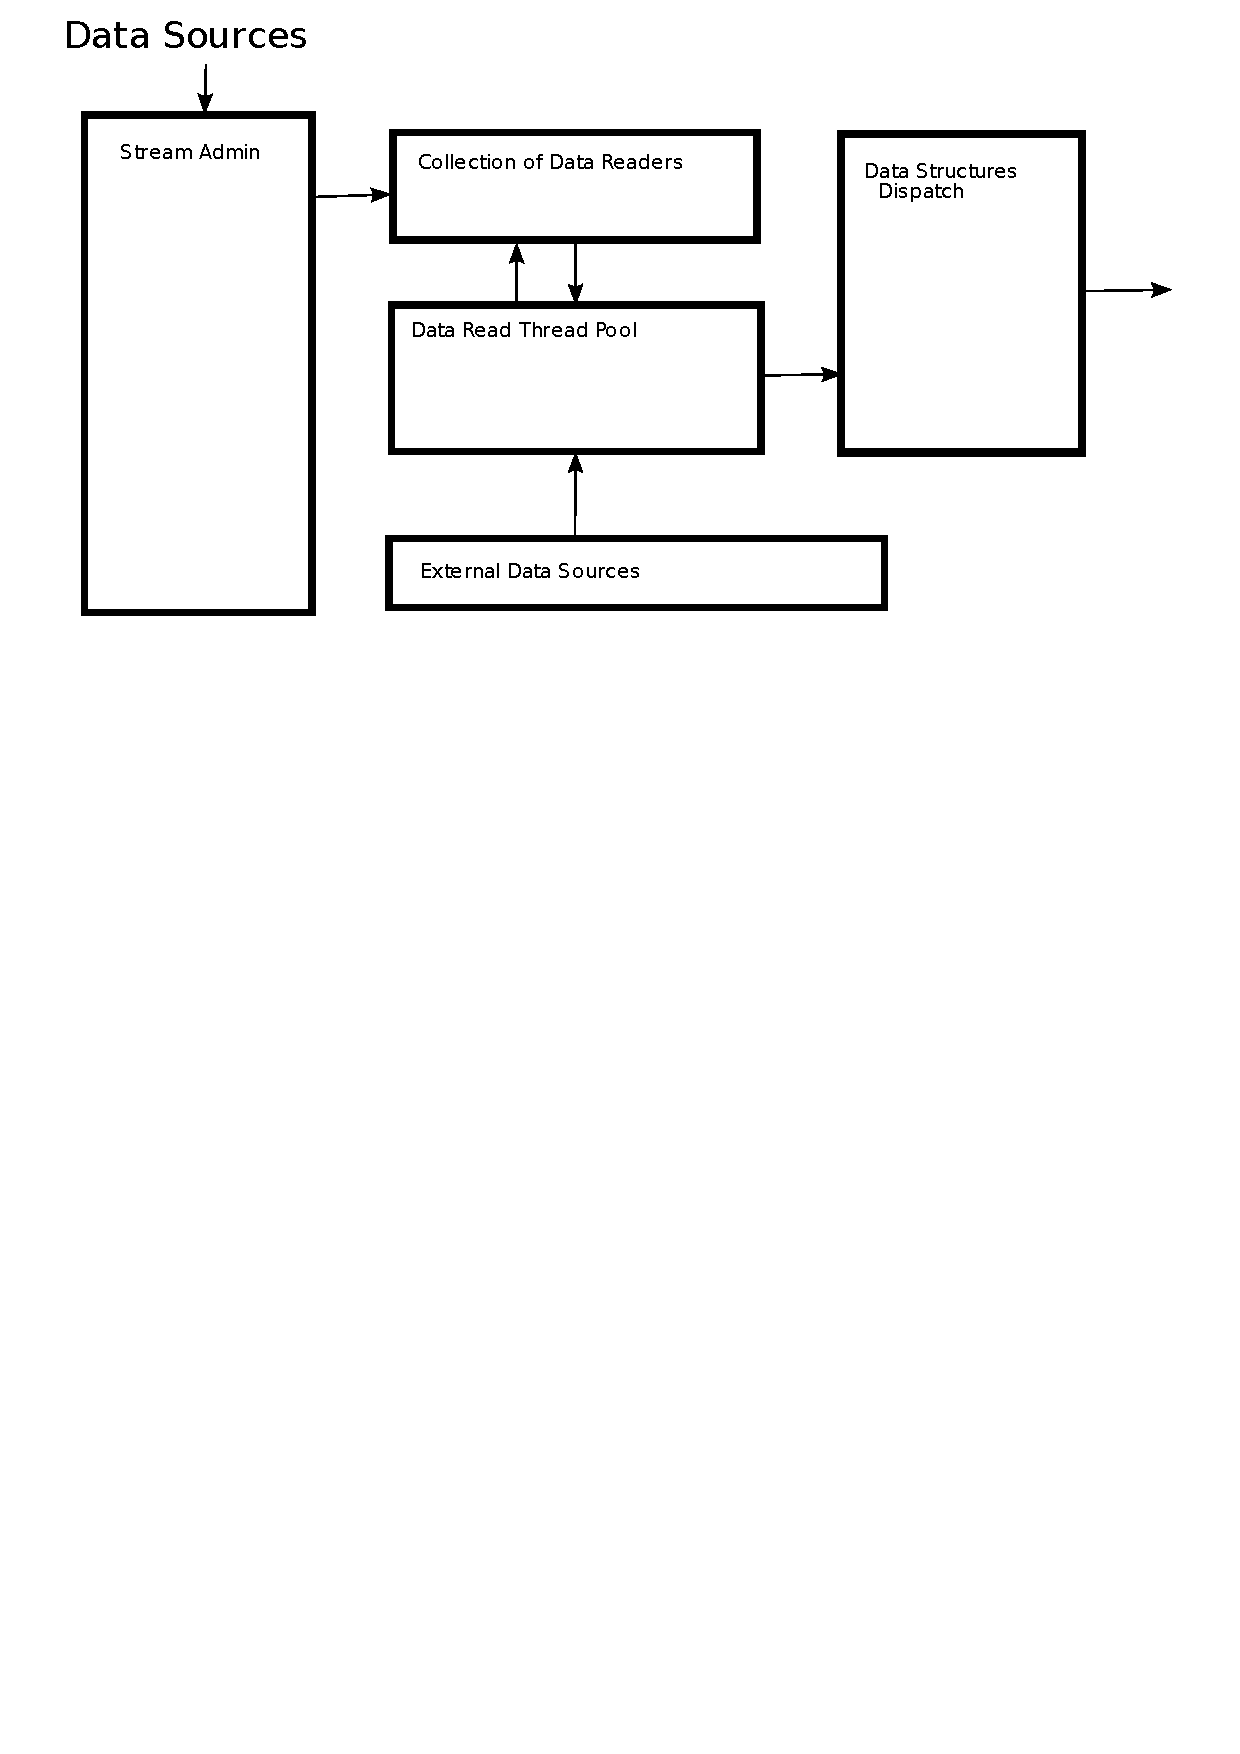
\includegraphics[width=5.00in]{../figures/DataSources.pdf}
  \caption{Data Sources Management.}
  \label{DataSourcePic}
\end{figure}

\subsubsection{Data Sources Admin}

Data Sources Admin provides interface to install new Data Sources.

\begin{verbatim}
class DataSourcesAdmin
{
	DataSourcesAdmin(InputBufferInterface*);
    addDataSource(sourceID, SourceReader, DataAdaptor);

	DataDispatcher;
    DataSourcesManager;
	InputBufferInterface*;

}
\end{verbatim}
 
\noindent It also creates Data Dispatcher and Data Sources Manager.

These interface is needed by the compiler to install new data sources upon users request. When add Data Source is initiated

\begin{itemize}
	\item Data Adaptor is inserted into a Data Dispatcher
	\item Data Source reader added to Data Sources Manager. It in turn adds it to a queue of available data sources to be read from.
\end{itemize}

%Data Sources Admin receives two function handles one to a data Reader and another one for a Data Adaptor from a Compiler. First Admin locks Data Adaptors and inserts a new Data Adaptor. Then Admin locks Data Readers Queue  and a handle is inserted. Each Data Readers handle implements a method \emph{readNext()} for reading data from some data source (typically a socket or a file).

%\begin{itemize}
%	\item {\tt rawDataTuple getNext(); // user defined function - provided}
%\end{itemize}

%\noindent The {\tt rawDataTuple} is a pair {\tt <size, bit-string>}.

%The Reader extracts the informations from either a file or a socket. Reader's communication with the outside world is in a standard format. On a read request, Reader first reads a header containing the information about the message followed by the message itself. For now we assume that a header is an integer containing the number of byte to be read. Once the read is completed the size and message are forwarded to Data Structures Dispatch.

\noindent \emph{TODO: expand this into a section with the full description of Readers input formats}.

%\noindent Data Sources Admin class contains the following:



\subsubsection{Data Readers Thread Pool}

Data Readers Thread Pool is a collection of identical threads. Each thread is responsible for getting a reader from the queue of Data Readers, executing a \emph{readNext()} message, collecting the message {\tt rawDataTuple} and sending it to Data Structures Dispatch together with the ID of a Reader.

The class of the Data Readers Thread Pool looks as follows:
\begin{verbatim}
class DataReadersPool
{
	void Run();
	
    list<thread>            runningThreads;
    DataReadersQueue        sources;
    DataDispatch            outputBuffer;
}
\end{verbatim}

\noindent The class of Data Readers Thread Pool contains a Data Readers Queue:

\begin{verbatim}
class DataReadersQueue
{
	functionHandle  getNextReader();
	void            putNextReader(functionHandle);
	
    queue<functionHandle>  sources;
}
\end{verbatim}

\noindent and a Data Dispatch.

\subsubsection{Data Dispatch}

Data Dispatch receives an ID identifying each Data Source and a message read by the reader. 

\begin{itemize}
	\item {\tt dispatchNext(readerID, rawDataTuple);}
\end{itemize}

Based on the ID of a reader Dispatch Calls for on an appropriate Data Adaptor to convert the incoming {\tt rawDataTuple} message into a structure needed by the query. The structured tuple is then sent to an appropriate set of queues in the Data Queue for Processing. The {\tt structuredTuple} is a pair {\tt <size, bit-sequence>} such that the bit sequence can be interpreted by the query. 

\begin{verbatim}
class DataDispatch
{
	
	void dispatchNext(readerID, rawDataTuple);

private:
    void sendData();
	
    DataAdaptors;
    InputBuffer*;
}
\end{verbatim}

\noindent Data Adaptors map is a separate class just like Data Readers Queue

\begin{verbatim}
class DataAdaptors
{
    functionHandle  getAdaptor(sourceID);
    void            addAdaptor(sourceID, functionHandle);

    map<sourceID, functionHandle>;
	
}
\end{verbatim}
\noindent They are needed to be separated into classes to deal with concurrency.

\subsection{Query Processor}

Query Processor is done mostly in Query Executor with a set of Query Threads each thread picks a query-datum pair from a pool of available pairs and processes it. As data comes in after been processed it is sent to the appropriate query. As soon as query receives a datum it becomes available for execution. The structure of query processor can be found in figure \ref{QueryProcessingPic}.

\begin{figure}
  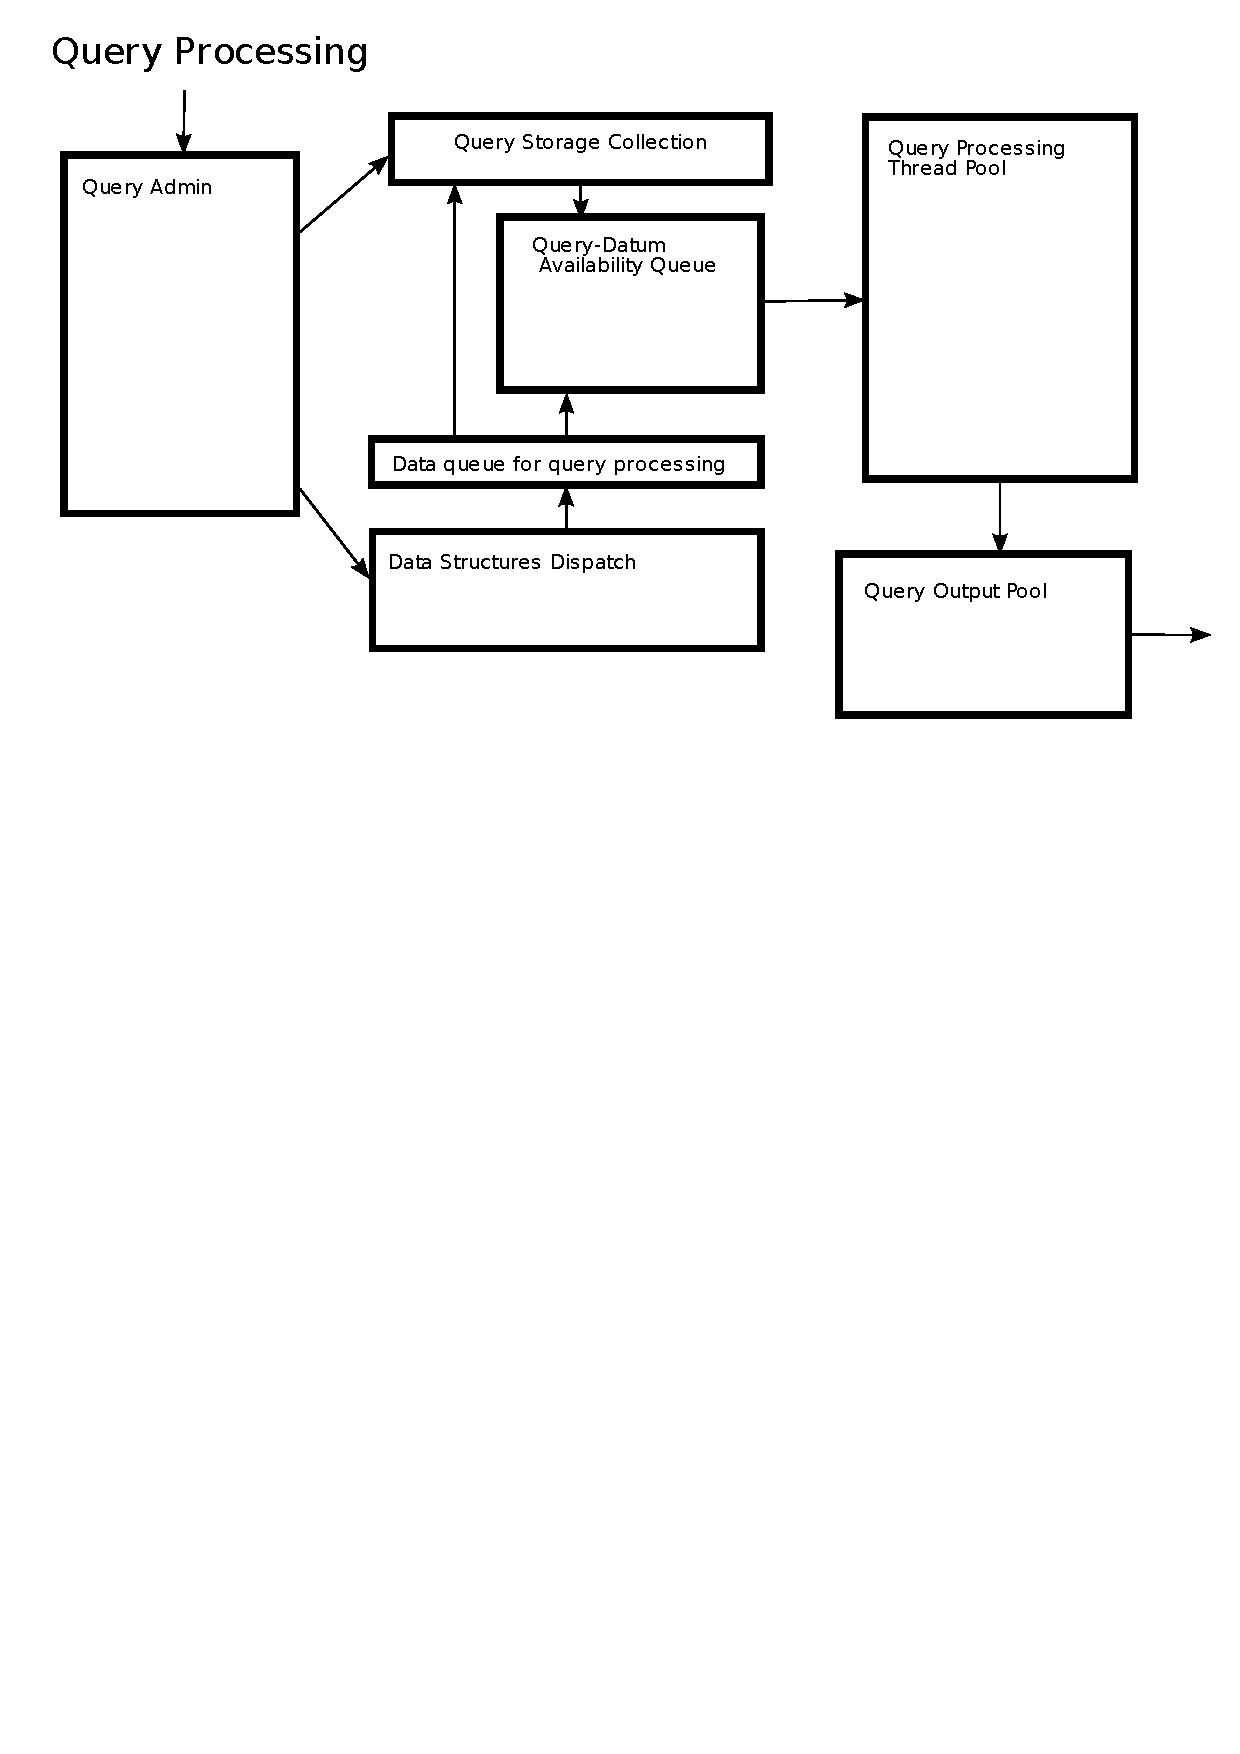
\includegraphics[width=5.00in]{../figures/QueryProcessing.pdf}
  \caption{Query Processing Management.}
  \label{QueryProcessingPic}
\end{figure}

\subsubsection{Query Admin}

Query Admin receives a function handle to a query. It also receives a list of the readers IDs for that query. Once the handle is received Admin locks Query Catalog and inserts the query there, then Query Results Queue is locked and updated to have an output queues for just inserted query. Finally Admin locks Query Tuple Queue and inserts and additional queue for data associated with the query. 

Query Catalog is a map containing query ID and a handler for that query. 

Query Admin class looks as follows
\begin{verbatim}
class QueryAdmin
{
    addQuery(queryID, functionHandle, list<int> ReadersID);

	queryCatalog;
	networkCatalog;
	QueryTupleQueue*;
	
}
\end{verbatim}

\subsubsection{Query Executor}

Query Executor consists of two inter dependent components: Input Buffer and Scheduler. Input Buffer stores data needed for query execution. Scheduler contains a set of threads which run one query at a time on data from Input Buffer. InputBufferInterface and SchedulerInterface are two classes which provide interface for InputBuffer andScheduler. 

\paragraph{Input Buffer}

Input Buffer is a class, which provides seamless access to the data and storage. It contains a queue per data source, each query when registered can get the data from those queues. When Input Buffer receives a new tuple from Data Dispatch, together with an ID of the data Source (in a format {\tt structuredTuple}), the new tuple is inserted into appropriate queue. If the tuple insert causes a query to be available a Scheduler is notified to add such a query for processing. If the query is already runable then the tuple is just inserted into the queue.

\noindent InputBufferInterface has the following structure:

\begin{verbatim}
class InputBufferInterface
{
    void                  addTuple(int sourceID, void * structuredTuple);
    void *                getTuples(int queryID);
    void                  addQuery(int queryID, int sourceID);
    void                  removeQuery(int queryID);
    void                  hasNext(int queryID);
    void                  removeTuples(int queryID);
	
}
\end{verbatim}

Input Buffer class has the following structure:

\begin{verbatim}
class InputBuffer
{
	InputBuffer(MemoryManager* Jim);
    void             addTuple(int sourceID, void * structuredTuple);
    void *           getTuples(int queryID);
    void             addQuery(int queryID, int sourceID);
    void             removeQuery(int queryID);
    void             hasNext(int queryID);
    void             removeTuples(int queryID);
    void             addScheduler(SchedulerInterface* sch);

	MemoryManager*                     Jim;
	Scheduler*                         schedulingQueue;
	map<sourceID, list<TupleQueue*> >  sourceAccess;
	map<queryID, list<TupleQueue*> >   queryAccess;
	map<sourceID, list<queryID> >      availableQueries;
	
}
\end{verbatim}

\noindent Here we refer to {\tt queryID} as to an ID of a query coupled with data source. This ID is created in Query Catalog. The purpose is to make a direct link between a query and source and hide the details of dealing with several sources for each query inside the Scheduler.

Interface function {\tt addTuple(sourceID, structuredTuple)} is called by the Data Dispatch to add a new data item. Functions {\tt getTuple(queryID), hasNext(queryID)} and{\tt removeTuples(queryID)} are required to extract tuples available for the query to be executed as well as for cleaning up queues. Functions {\tt addQuery(int queryID, int sourceID)} and {\tt removeQuery(queryID)} are needed by Query Admin to insert or remove a new queries. 

To enable this functionality we need to consider concurrency and efficiency. 

\subparagraph{Concurrency:} Each queue can be accessed by several queries and only one data source. Locking needs to be enabled to prevent overlapping on insertion and deletion. Reading data should be available to all queries simultaneously. SharedTupleQueue provides this controls internally for each queue. Since there is no race between different queues there is no need to create concurrency between them.

\subparagraph{Efficiency:} The main inefficiency comes form the fact that data from one data source needs to be accessed by several queries. If we adopt a simple model (case A) where each query has its own set of queues for each of the required sources, we have inefficiency of coping data to each such queue. The benefit of such model is simplicity of implementation and use. Also the concurrency mechanisms are simple and very efficient. Another model (case B) is to have only one queue for each data source. In this case each queue will need to keep track of which query requires what item from this queue as well as removal of used tuples. The benefit of this method is simpler storage method and memory management. Both approaches can be supported. We can hide all this details into the implementation of queue and Input Buffer. By requiring the following specification:

\noindent Case A:
\begin{verbatim}
class QueryTupleQueue
{
    QueryTupleQueue(MemoryManager*);
	
	void              addTuple(structuredTuple);
	void *            getTuples();
	bool              isEmpty();

	queue<StructuredTuple>   tuples;
}
\end{verbatim}

\noindent Case B:
\begin{verbatim}
class SharedTupleQueue
{
    SharedTupleQueue(queryID, MemoryManager*);

	TupleQueue*       join(queryID);
	void              removeQuery(queryID);
	
	void              addTuple(structuredTuple);
	structuredTuple   getTuples(queryID);
	bool              isEmpty(queryID);
	void              removeTuples(queryID);
	
	map<queryID, pointerToPositionInQueue>     nextTuple;
	queue<SharedTuple>                         datum;
	MemoryManager*                             memMan;
}
\end{verbatim}

\begin{verbatim}
struct SharedTuple
{
    int              beenAccessed;
    StructuredTuple*  datum;
}
\end{verbatim}

We decided to adopt Case B due to the savings of memory and copying of data tuples.

When a new query is inserted into Query Admin, it calls on Input Buffer with {\tt addQuery(queryID, int sourceID)} for each data source (remember that queryID is an ID indicating query source connection and can be mapped to a real query in Query Catalog). If the source is not present (we can find it though {\tt map<sourceID, list<TupleQuery*> >}) we create a new Tuple Queue, but if it is we call {\tt join(queryID)}. {\tt join(queryID)} in case A will create a new TupleQueue and return a pointer to it or in case B it will return a pointer to this queue and change internal structure to accommodate a new query. ({\tt removeQuery(queryID)} is a reverse. It is either a destructor or changes internal representation). When a new tuple comes in, by the call of {\tt addTuple(sourceID, structuredTuple)} in InputBuffer.

\subparagraph Memory Manager: to increase efficiency we want to allocate storage for the tuples in pages. Memory Manager provides an interface to receive and address of a new page and gets an old freed up page back. The writing to the page as well as management of allocation within a page will happen inside Shared Tuple Queue. 

\begin{verbatim}
class MemoryManager
{
    void * getPage();
	void   returnPage();
}
\end{verbatim}

\noindent To ease the management of page memory class Pages Manager is created. It keeps track of all relevant information needed to allocate space for new tuples.

\begin{verbatim}
class PagesManager
{
    PagesManager(MemoryManager*);
    void * getSpace(int* size);
    void   free(void* position, int* size);
    
}
\end{verbatim}

\paragraph{Scheduler}

Scheduler's job to execute a query on an appropriate data tuples. This goal is achieved by having a set of identical threads execute jobs. Each thread is responsible for picking up a query from Runable Query Queue. Then thread runs a query on the data tuple from Input Buffer. The results are put into a Query Results Queues; into a set of queues for the users which are interested in the results of this query. 

The execution flow within each thread is as follows:

\begin{verbatim}
get a queryID from RunableQueryQueue;
get data a set of data tuples from Input Buffer;
get a handle to a query function from QueryCatalog;

run Query on a set of tuples;

release data in InputBuffer;

if more data for query 
	put query onto RunableQueryQueue;

put results to QueryResultsQueue;
Repeat...

\end{verbatim}

Scheduler class contains the following:

\begin{verbatim}
class Scheduler
{
	Scheduler(QueryCatalog*);
    void       Run();
    void       addRunableQuery(querySourceID);

    RunableQueryQueue   availableQueries;
    list<thread>        executionThreads;
    InputBuffer *       readyData;
	QueryCatalog*       queryHandles;
	
}
\end{verbatim}

Function {\tt addRunableQuery(querySourceID)} is used by Input Buffer to check if the current query is available for running and if it is not add it to ready for a set of Runable Queries.

\noindent With RunableQueryQueue as follows:

\begin{verbatim}
class RunableQueryQueue
{
    
    queryID        nextQuery();
    void           addQuery(queryID);
    void           removeQuery(queryID);
    bool           isActive(queryID);

    queue<queryID>    readyQueries;
	
}
\end{verbatim}


\subsubsection{Query Results Queue}

Query Results Queue implements a server, where each client upon connection indicates a set of queries they are interested in.

\begin{itemize}
	\item {\tt userDataStructuresDispatch(userID, Query ID list);}
\end{itemize}

\noindent The server creates a map of query IDs and query results for each client. When a query produces an output, it is sent to the Query Result Queues. In the Result Queues the query results are dispatched to the appropriate queues.

\begin{itemize}
	\item {\tt queryDataStructuresDispatch(queryID, queryMap);}
\end{itemize}

\noindent When a client needs a new piece of information it sends a request to the server with the ID of a query it is interested in and the number of tuples it needs. Server returns the results of the query indicated by the ID and the tuples it produced. 

Query Result Queues implements two ways for the users to access data. One is when a user asks for a complete query result and another is when a client asks for an cursor to query results.

Query Result Queue class is:

\begin{verbatim}
class SchedulingQueue
{
    
	map<queryID, queryResult>
	
	getFullQueryResult(clientID, queryID);
	
	startCursorResult(clientID, queryID);
	
}
\end{verbatim}








\section{AlgoTrader}

AlgoTrader is an application of DBToaster Runtime to the domain of Stock Exchange and Algorithmic Trading. It consists of two parts an automatic Stock Trading Simulator and a platform for development and execution of Automatic Stock Trading Algorithms. The purpose of AlgoTrader is to demonstrate the potential of DBToaster Runtime to process time critical, expressive queries over streaming data. To demonstrate the power of Runtime two components are needed: a source(s) of streaming data and an application(s) that needs to run queries over the data from the sources. Exchange Server Simulator provides a source of continuous stock transactions between interested parties. AlgoEngine implements a set of trading strategies each strategy utilizes results of a query over the data from Exchange Server Simulator, from a DBToaster Runtime to make a decision about purchase/sell of stocks. 
  

\subsection{Exchange Server Simulator}
Exchange Server Simulator (ESS) is designed to reproduce the behavior of Electronic Crossing Networks (ECN). ECN facilitates stock exchanges between different parties connected to the network. Each ECN provides certain data to the subscribers. For now we limit ourselves to the complete knowledge about the changes in the stock order books. An order book for a stock contains all sell (ask) and buy (bid) request for such stock. These data is distributed to all the subscribers of the network as a constant stream of updates to the order book. The current implementation of Exchange Server Simulator works only with one stock. 

Each Order Book consists of an Asks Book and Bids Book. Asks Book contains sell requests, Bids Book - buy requests. Each ask/bid requests is transmitted to all the subscribers. If two requests are matched the results of such a match are transmitted as well. 

The main difference between a real ECN and a Simulator, is a simulator's ability to replay the exchanges made at some earlier date and incorporate exchanges made by trading algorithms into this stream. 

We implemented ESS to support two types of clients: readers and writers. Reader clients constantly listen to the stream of messages without placing any order. Writer clients only place orders and interact with the Simulator to get the information about just placed order (like order ID). The detailed implementation of ESS is as follows.

\subsubsection{Exchange Server}
ExchangeServer creates a server on local host and indicated port and handles all incoming client connections. Each connected client is handled in its own thread (ExchangeThread). ExchangeServer also creates one client (DataThread). This client is responsible for reading historical data from a file, connecting to a server and transmitting the data to the server. The server also creates structure for storage of order book information. It is shared by all clients.

The basic structure of Exchange Server is as follows:
\begin{verbatim}
open(Server_Socket);
SynchronizedBooks DataBook;
DataThread historical_data(inputDataFile.cvs);
historical_data.run();

while (Server_socket.listen())
{
	get(client);
	run(client, DataBook);
}
\end{verbatim}


\subsubsection{Exchange Thread}
When a client connects to an ESS, it creates an ExchangesThread to handle client needs. All ExchangesThreads share order book storage structure DataBoo. They also share a list of all connected clients.

The communication protocol between a client and server is as follows: 

The first message a server expects form a thread is a client type.

\begin{tabular}{|l|l|}
  \hline
  \multicolumn{2}{|c|}{Client type} \\
  \hline
  0 & Writer\\ \hline
  1 & Reader \\
  \hline
\end{tabular}
\\
\\*
\emph{Writer} clients are designed to send data and receive messages only as response to their transactions. \emph{Reader} clients receive all ongoing transactions but do not to send the messages themselves.

The messages from clients are coming in the pre-specified format:

\begin{verbatim}
long time;
int  order_id;
int  brokerage_id;
char action;
int  volume;
int  price;
\end{verbatim}

Where \emph{time} indicates the time when requests arrived to the server, \emph{order\_id} a unique identifier for each order arrived to ESS, \emph{brokerage\_id} ID identifying a company which placed a request for an order, \emph{action} one of several actions (buy, sell, cancel) described below, \emph{price} and \emph{volume} are price and amount of the stocks to be bought/sold. 

Several action can possibly occur:

\begin{tabular}{|l|l|}
  \hline
  Request & Action \\ \hline
  'B' & buy request, check ask book for match if no add to bid book \\ \hline
  'S' & see request, check bid book for match if no add to ask book \\ \hline
  'D' & delete request for an appropriate book if one exists \\ \hline
  'X' & cancel order remove trade request from appropriate book\\ \hline
  'E' & change request, generated by server \\ \hline
  'F' & order fulfilled, generated by server \\
  \hline
\end{tabular}

'B', 'S' and 'D' actions can come from any of the clients (to buy or sell stocks or delete request). Actions 'E', 'F' and 'X' are generated by the server as a result of a partial match, match or delete request. 

Each transaction and its consequences are announced to all Reader clients as well as to Writer client which initiated a transaction. 

The basic operation of each Exchange Thread is:

\begin{verbatim}
while (listen(request)){
	messages=DataBook.update(request);
	foreach(Reader)
	 send(messages);
}
\end{verbatim}

% the first  message showing an interest in exchange ExchangesThread checks if there is an appropriate match in the data structures (i.e. if some one wants to sell some amount of stocks the thread will look if someone wants to buy stocks at the given price), if so the match is executed if not the request is stored in the data structures. The results and the transaction are announced to all the connected clients. 

\subsubsection{Synchronized Books}
SynchronizedBooks is a shared data structure for storage of order books information. It is shared between all clients. Each client can add/remove/modify bid/ask requests. SynchronizedBooks contains two SortedBooks. SortedBook is a structure that has properties of a sorted set and a hashtable. (The data is sorted by data values and can be accessed using keys).

When a sell/buy request is inserted into SynchronizedBooks, the data structure tries to find a matching buy/sell request. If a matching request is found an update message is generated in addition to sell/buy request. The update message contains information about the fact that one or both of the orders are partially/fully satisfied. The exchange message is of the form:


\begin{tabular}{|l|l|}
  \hline
  Action & Meaning \\ \hline
  'E' & order number, update amount \\ \hline
  'F' & order was executed in full \\

  \hline
\end{tabular}


SynchronizedBooks utilizes Order\_tuple to store each individual bid/ask request in SortedBooks. Stream\_tuple is used to generate as a communication message to be sent to clients.


\subsubsection{Historical Data}

ExchangeServer is capable of using historical data flow stock trades between real clients in addition to the transactions executed by Writer clients. ESS uses DataThread to extract historical data from a file and transmit it to server. DataThread can be started at any point during the execution by a server (for example, once there is a client connected to the server). DataThread reads a historical trace file in a .cvs format and transmits each message to the server as if it was a real request. DataThread does not dustings between client and server actions and transmit all of them as if they were requests of some client. ExchangeThread distinguishes orders coming from historical data and from live clients by the message data. Historical data contains order ID and timestamps for all the orders. Writer clients have 0 in those fields (except delete).  


\subsection{Algorithms Engine}

Algorithms Engine is an application designed to emulate actions of a hedge fund. It implements a set of trading algorithms. Each trading algorithm runs a query over the data produced by Exchange Server Simulator. Based on this information an algorithm makes a decision whether to buy or sell stocks. Those requests go directly to ESS. 

Algorithms Engine has two connections to ESS. The first connection is a writer client for sending ask/bid requests to the server. The second connection is a reader client to monitor the results of exchanges. The second connection notifies Algorithms Engine when and if ask/bid request have been executed. 

There are two concurrent execution paths inside Algorithms Engine. The first path creates a reader client to ESS and starts listening to the update stream. Each order on a stream is compared to a set of internal requests. If an incoming data is about one of the internal requests. The request is modified and appropriate statistics are changed. The second path creates one writer connection to ESS and a client connection to DBToaster Runtime. This path starts by initiating all of the trading algorithms. Each of the trading algorithms runs (or uses results of) a query over the data produced by ESS. These queries are executed by Runtime. The results of each query are used by Algorithms Engine to extract data for trading algorithms. When data is available, trading algorithms use it to determine whether to place ask/bid order. This process repeats continuously. 

%Algorithm Engine code developed by the end users. The code makes use of DBToaster Runtime to query the continuous data from input streams specified by the users. The query results are then processed by user defined algorithms to achieve their goals. 

%In our example Algorithmic Engine creates and runs a set of monitoring queries for the stock trading depending on the results of the queries and the internal mechanics - algorithms decide to buy or sell stocks on a NASDAQ Trading Exchange Simulator.

\subsubsection{Algorithms Engine}

AlgorithmsEngine class contains all the trading algorithms, a connections ESS and a connection to DBToaster Runtime. On initiation it creates a Reader connection to ESS. A trading algorithm can be added at any time during execution. 

\begin{verbatim}
class AlgorithmsEngine
{
    AlgorithmsEngine();
    void runAlgos();
    void addAlgo(AlgoInterface * algo);

private:
    void getData();
    
    list<AlgoInterface*> my_algos;
    DataCollection       data;
    OrderManager         manager;
	
}
\end{verbatim}

DataCollection is an interface to DBToaster Runtime. It contains query results. OrderManager contains statistics for each algorithm and order requests from all algorithms. 

The execution cycle of \emph{runAlgos()} is

\begin{verbatim}
void runAlgos()
{
    getData();
    
    foreach algo in my_algos
        requests=algo->run(requests);
    
    manager.handle(requests);
}
\end{verbatim}

Where requests is a set of order requests generated by the algorithms.

%Algorithmic Engine interacts with environment in three different ways. First of all the Engine needs to receive  the information from from DBToaster runtime. This interaction is unavoidable since the Engine needs the results of the queries. Another interaction which needs to be added is the way to specify the information stream received by a DBToaster runtime. This information needs to be passed the the Runtime in the form of c++ code for the Runtime to compile. Another optional source of interaction is infulencing the enviroment. In our example is the Engine's capability to add/remove stock requests from the Exchange Server. 

\subsubsection{Order Manager}
OrderManager is an interface with ESS. 

\begin{verbatim}
class OrderManager
{
    void sendOrders(function handler, deque<AlgoMessages*> messages);
    void startReading(boost::asio::io_service& io_service)
    void processOrder(DataTuple & tuple);
    
private:
    WriterConnection *             writer;
    WriterConnection *             reader;

    ptr_map<LocalID, DataTuple>   dataOrders;
    ptr_map<OrderID, LocalID>     orderIDtoLocalId;
    ptr_map<LocalID, DataTuple>   executedOrders;
}
\end{verbatim}

Order Manager has two connections to ESS: a writer and a reader clients. Each of them runs in different thread. Reader client is invoked by \emph{startReading} function. It creates a loop where \emph{processOrder} is called repeatedly. Writer client is invoked by \emph{sendOrder} function. It gets a list of order requests form trading algorithm adds them to \emph{dataOrders} list and sends them to ESS. \emph{processOrder} function in turn checks \emph{dataOrders} if it contains incoming message \emph{tuple}. If it does the update to \emph{dataOrders} is made and as well as to the statistics for each algorithm.

\emph{executedOrder} stored all the completed requests. \emph{orderIDtoLocalId} is a map from Server's identifier for each order to internal identifier of the Order Manager for each order.


\subsubsection{Data Collection}
DataCollection class provides high level interface to ESS. It contains a \emph{ToasterConnection}. 

\begin{verbatim}
class DataCollection
{
    void ReadSOBI();
    void update();
    ToasterConnection toaster.
}
\end{verbatim}

Toaster Connection is a thrift client to DBToaster Runtime. It collects results of queries from Runtime. 

Data Collections also contains a number of read and update functions to collect and extract needed data from query results.

%\subsubsection{Data Stream}

%There are two interactions with outside systems needed to be implemented by the user. The first interaction is with DBToaster. A system needs to pull information from the DBToaster runtime. \emph{TODO description of the the pulling mechanism}.

%Another interaction, which needs to be passed to the DBToaster Runtime, is a way for Runtime to access the data streams relevant to the Engine and over which the queries needed to be post. This information is specified as a C++ code which is sent for the compilation to the Runtime to be added to the system.

%\subsubsection{External Influence}

%If the Engine implements interactive process, which needs to access outside processes or interact (influence) them then this is interactivity needs also to be added. In our example Algorithmic Engine can buy and sell stock on our Exchange Simulation Server. Thus acting like one of the clients of the server. \emph{TODO describe the system in more details}

\subsubsection{Algorithms}

Algorithms are the main interest of Algorithms Engine and a driving force for DBToaster Runtime. Each Algorithms makes a decision about buying or selling stocks based on the information from ESS. Relevant information for each algorithm can be extracted by running a query over Order Books of ESS. DBToaster Runtime provides the functionality to do so. 

Currently there is a set of algorithms implemented by Algorithms Engine. 

\paragraph{Simple SOBI}

Static Order Book Imbalance (SOBI) is a strategy of comparing the difference between last known stock price and volume-weighted average price (vwap) of stock in each order book. For example, a much greater difference between last price and vwap of an ask book to that of last price and vwap of bid price indicates that sellers do not support current price and that price has a great chance of rising. (The reverse also works.)

Simple SOBI strategy looks at this imbalance and when one value is four times greater than another, simple SOBI buys/sells a fixed number of stocks at a current price.

\paragraph{Volatile SOBI}

Volatile SOBI is a derivation of simple SOBI. It additionally takes into account information about price's standard deviation. The strategy buys/sells stocks when the difference between vwap and last price is greater than standard deviation.

\paragraph{Timed SOBI}

Timed SOBI is a strategy similar to Simple SOBI. It looks at an average timestamp of the top orders in each order book. The shift to an older values of time stamps indicates lessen support of the current price in this order book. Appropriate buy or sell order is generated for a fixed number of shares and at current price. 

\paragraph{Market Players} 

This strategy creates a query over both Order Books. This query looks for all traders which try to sell and buys stocks at the same time. In particular it looks for cases when a trader wants to sell small amount of stocks at a price a little bit higher than a current price. And the same trader wants to buy a big amount of stocks at a price much lower then current price. The strategy will place a sell order just below the sell order of this trader. The revers of this strategy is also executed.
\\
\\
Timed SOBI and Market Players are not yet operational. At the moment both of them are unsupported by the Runtime.

%This is the part which is the most relevant to the user and will vary from system to system. In out example we encoded the learning and trading strategies for NASDAQ stock exchange. \emph{TODO describe the system in more details}

\subsubsection{Query Creator}

At the moment Algorithms Engine does not provide a support write SQL queries and send them for addition to DBToaster Runtime. This functionality needs to be added. This will require additional support from both Runtime and Toaster Connection.

%Queries posed to the DBRuntime can come from various sources they can either be predefined by the user system or written and modified dynamically. In order to be active they need to be passed to the Runtime where they are compiled and added to stream observations. \emph{TODO describe the process more}



\end{document}





